% !TEX encoding = UTF-8 Unicode
\documentclass[
10pt,
aspectratio=169,
]{beamer}
\setbeamercovered{transparent=10}
\usetheme[
%  showheader,
%  red,
  purple,
%  gray,
%  graytitle,
  colorblocks,
%  noframetitlerule,
]{Verona}

\usepackage[T1]{fontenc}
\usepackage[utf8]{inputenc}
\usepackage{lipsum}
%%%%%%%%%%%%%%%%%%%%%%%%%%%%%%%
% Mac上使用如下命令声明隶书字体,windows也有相关方式,大家可自行修改
%\providecommand{\lishu}{\CJKfamily{zhli}}
%%%%%%%%%%%%%%%%%%%%%%%%%%%%%%%
\usepackage{tikz}
\usetikzlibrary{fadings}
\usetikzlibrary{shapes.geometric}
\usetikzlibrary{positioning}
%\tikzset{
%  every overlay node/.style={
%    draw=black,fill=white,rounded corners,anchor=south west,
%  },
%}
% Usage:
% \tikzoverlay at (-1cm,-5cm) {content};
% or
% \tikzoverlay[text width=5cm] at (-1cm,-5cm) {content};
%\def\tikzoverlay{%
%   \tikz[baseline,overlay]\node[every overlay node]
%}%
\tikzset{
  every overlay node/.style={
    anchor=north west,
  },
}
\def\tikzoverlay{%
   \tikz[baseline,overlay]\node[every overlay node]
}%


\newenvironment{smallgreentext}{\scriptsize\color{green}}{\par}
\newenvironment{smallbluetext}{\scriptsize\color{blue}}{\par}
\def\checkmark{\tikz\fill[scale=0.4](0,.35) -- (.25,0) -- (1,.7) -- (.25,.15) -- cycle;}

%
%\setbeamertemplate{sections/subsections in toc}[ball]
%\usepackage{xeCJK}
\usepackage{adjustbox} % Shrink stuff
\usepackage{listings}
\usepackage{caption}
\usepackage{subcaption}
\usefonttheme{professionalfonts}
\def\mathfamilydefault{\rmdefault}
\usepackage{amsmath}
\usepackage{multirow}
\usepackage{booktabs}
\usepackage{bm}
\setbeamertemplate{section in toc}{\hspace*{1em}\inserttocsectionnumber.~\inserttocsection\par}
\setbeamertemplate{subsection in toc}{\hspace*{2em}\inserttocsectionnumber.\inserttocsubsectionnumber.~\inserttocsubsection\par}
\setbeamerfont{subsection in toc}{size=\small}
\AtBeginSection[]{%
	\begin{frame}%
		\frametitle{Outline}%
		\textbf{\tableofcontents[currentsection]} %
	\end{frame}%
}

\AtBeginSubsection[]{%
	\begin{frame}%
		\frametitle{Outline}%
		\textbf{\tableofcontents[currentsection, currentsubsection]} %
	\end{frame}%
}

\title{Propuesta: metodolog\'ia}
\subtitle{Estructuraci\'on y realizaci\'on de la propuesta}
\author[L.M.]{Luis Alejandro Morales, Ph.D.}
\mail{email: lmoralesm@unal.edu.co \\ url: \url{https://lamhydro.github.io}}
\institute[UNAL]{Facultad de Ingenier\'ia, Departamento de Ingenier\'ia Civil y Agr\'icola\\
Universidad Nacional de Colombia, Bogot\'a}
\date{\today}
\titlegraphic[width=3cm]{logo_01u}{}

%%%%%%%%%%%%%%%%%%%%%%%%%%%%%%%%
% ----------- 标题页 ------------
%%%%%%%%%%%%%%%%%%%%%%%%%%%%%%%%
% New commands
\newcommand{\gi}{\texttt{Git}}
\newcommand{\gih}{\texttt{GitHub}}
\newcommand{\co}[1]{\alert{\textbf{\large \texttt{#1}}}}

\begin{document}

\maketitle

%%% define code
\defverbatim[colored]\lstI{
	\begin{lstlisting}[language=C++,basicstyle=\ttfamily,keywordstyle=\color{red}]
	int main() {
	// Define variables at the beginning
	// of the block, as in C:
	CStash intStash, stringStash;
	int i;
	char* cp;
	ifstream in;
	string line;
	[...]
	\end{lstlisting}
}
%%%%%%%%%%%%%%%%%%%%%%%%%%%%%%%%
% ----------- FRAME ------------
%%%%%%%%%%%%%%%%%%%%%%%%%%%%%%%%

%----
\section{Metodolog\'ia}
\begin{frame}{Metodología}
\begin{itemize}
\item Se describe lo que se hizo. No incluir informaci\'on referente a m\'etodos o procedimientos no utilizados. 
\item \alert{Relativamente fácil de escribir porque no requiere interpretaciones.}
\item Comúnmente conformada por:
\begin{itemize}
\item Caso de estudio. E.j. Lugar geogr\'afico.
\item Informaci\'on: E.j. Series temporales de precipitación del IDEAM.
\item Métodos anal\'iticos/num\'ericos. E.j. Solución de las ecuaciones de Saint-Venant.
\item Métodos estadístico. E.j. Regresiones multivariadas.
\item Experimentos. En campo o en laboratorio.
\item Diseños de instrumentos.
\end{itemize}
\end{itemize}
\tikzoverlay[text width=8.5cm] at (1.5cm,-0.5cm) {
\centering
\begin{smallbluetext}
\large Un lector debe ser capaz de reproducir lo que se realiz\'o de acuerdo a lo descrito en la metodolog\'ia
\end{smallbluetext} 
};
\end{frame}

\begin{frame}{Ejemplos de metodologías}
\begin{columns}
\column{0.5\textwidth}
\textbf{Modelos regionales para la estimación de caudales medios anuales y de crecientes en la Amazonia y la Orinoquia Colombiana} (\alert{Investigaci\'on})
\centering
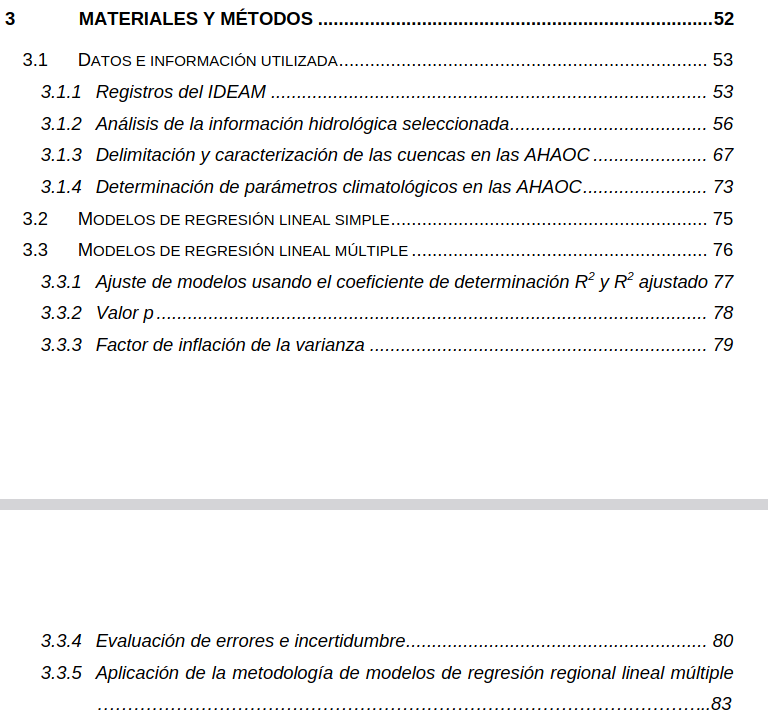
\includegraphics[width=0.8\textwidth]{metof1.png}
\column{0.5\textwidth}
\textbf{Evaluación del manejo del agua en la extracción y producción de hidrocarburos con miras a la definición de alternativas de tratamiento y reúso} (\alert{Profundizaci\'on})
\centering
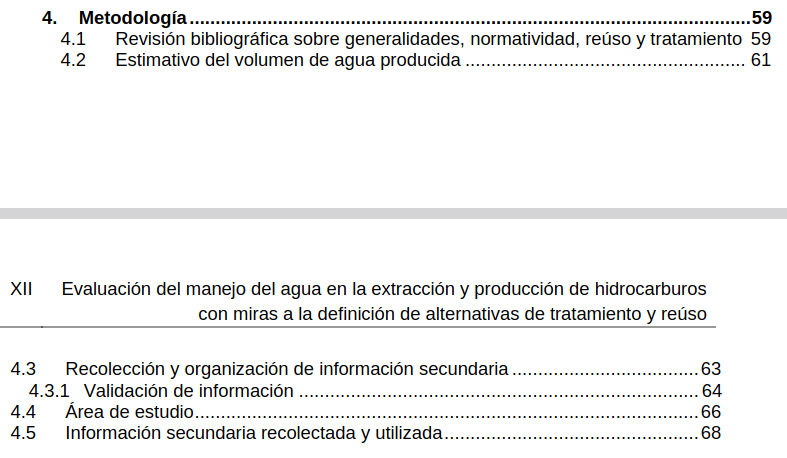
\includegraphics[width=\textwidth]{metof2.png}
\end{columns}
\end{frame}


\begin{frame}{Metodolog\'ia}
Escoger un art\'iculo de investigacion sobre su idea de trabajo y leer la metodologia para:
\begin{itemize}
\item Metodos o modelos utilizados
\item Zona de estudio
\item Datos recopilados
\item Diseño de experimentos
\end{itemize}
\end{frame}




\end{document}


